\documentclass[tikz]{standalone}

\begin{document}
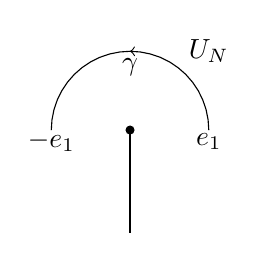
\begin{tikzpicture}
  \clip (-1.3, -1.3) rectangle (1.3, 1.3);
  \draw (0, -2) -- (0, 0);
  \draw[fill=black] (0, 0) circle (0.05);
  \draw[domain=0:180] plot ({cos(\x)}, {sin(\x)});
  \draw[->] (0.001, 1) -- (-0.001, 1.000);
  
  \node at (1, 1) {$U_N$};
  \node at (1, -0.15) {$e_1$};
  \node at (-1, -0.15) {$-e_1$};
  \node at (0, 0.8) {$\gamma$};
\end{tikzpicture}
\end{document}
